\section{Neo4j}
\begin{displayquote}
    \textit{\textbf{CAP:} CA - Konsistent med en høj tilgængelighed (ACID kompatibel)}
\end{displayquote}

Neo4j er en NoSQL databasetype, mere specifikt er det en graph database. Sammen med andre NoSQL databaser kan denne skaleres horisontalt \cite{graphfacelift}, og har en semi-struktureret datastruktur, der blandt andet gør det muligt at lagre forskellige formater af data. Graph databaser er pr. design lavet til data med store mængder af relationer, hvorfor det var oplagt at benytte sig af neo4j til lagring af information på og relationer mellem film, serier, skuespillere, forfattere osv. Eftersom al dette data deler mange relationer indbyrdes, eksempelvis har skuespillere relationer til de film og serier de medvirker i. En anden fordel ved denne database type er dens fleksibilitet vedr. dataformatet, hvilket på sigt kan ændre sig alt efter behov. Neo4J og graph databaser bruges dog ikke til at lagre selve mediet men man kan derimod have en attribut på en node i Neo4J der peger mod mediefilen \cite{graphmediafiles}.
\bigbreak
Til databasen er der udviklet to datamodeller: en for film og en for serier. Der er ikke udviklet datamodeller til skuespillere, instruktører eller manuskriptforfattere på grund af, at det er relationen mellem dem og filmen/serien der er vigtig. De to datamodeller ses på listing \ref{lst:movie} og \ref{lst:series}:

\begin{tcolorbox}
    \lstset{style=sharpstyle}
    \begin{lstlisting}[language={[Sharp]C}, caption={C\# MovieModel Class}, label={lst:movie}]
        public class MovieModel {
            public string Title { get; set; }
            public string ReleaseYear { get; set; }
            public string Description { get; set; }
            public string genre { get; set; }
            public List<string> actors {get; set;}
            public List<string> directors {get; set;}
            public List<string> writers {get; set;}
        }
    \end{lstlisting}
\end{tcolorbox}

\begin{tcolorbox}
    \lstset{style=sharpstyle}
    \begin{lstlisting}[language={[Sharp]C}, caption={C\# Seriesodel Class}, label={lst:series}]
        public class SeriesModel {
            public string Title { get; set; }
            public string ReleaseYear { get; set; }
            public string Description { get; set; }
            public string genre { get; set; }
            public List<string> actors {get; set;}
            public List<string> directors {get; set;}
            public List<string> writers {get; set;}
            public int seasons {get; set;}
        }
    \end{lstlisting}
\end{tcolorbox}
De to modeller ligner til forveksling hinanden meget, men serie modellen afviger fra MovieModel ved at have en ‘seasons’ attribut, der viser hvor mange sæsoner den respektive serie har. Hver serie og film node i databasen består af attributterne title, ReleaseYear, Description og Genre hvor serier også har Seasons. For actors, directors, writers og genre, så er disse ikke attributter direkte på noden, men derimod en node for sig selv hvor den specifikke serie eller film har en relation til. 

\subsection*{Struktur af noderne}
\begin{figure}[H]
    \centering
    
\includegraphics[scale=0.62]{graph_color.png}
    \caption{Farvekoder til neo4j.}
    \label{fig::graph_color}
\end{figure}
For at gøre det nemmere at gennemskue den data der ligger i neo4j, kan noderne inddeles efter en farvekode og størrelse. Mere relevante og overordnede noder som genre, film og serier bliver større, mens underordnede noder som episoder bliver små. 

\begin{figure}[H]
    \centering
    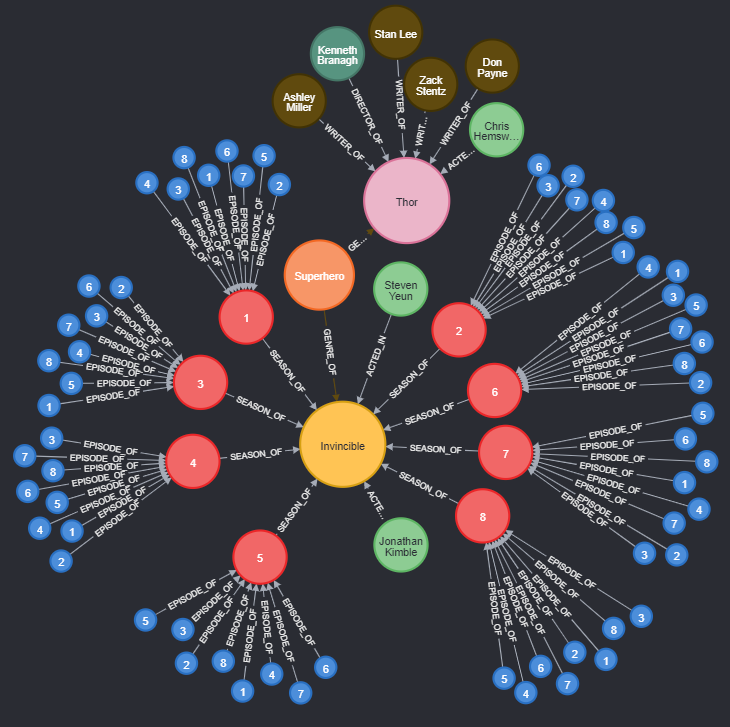
\includegraphics[scale=0.62]{graph.png}
    \caption{Film og serie tilknyttet til “Superhero” genren.}
    \label{fig::graph}
\end{figure}
På figur \ref{fig::graph} ses et udsnit af neo4j databasen, med en enkelt film og serie samt deres tilhørende børne-noder, som er inddelt efter farve som set på figur \ref{fig::graph_color}. Film og serier der bliver oprettet bliver knyttet til en genre, og derefter knyttes medvirkende til en film/serie. En serie har derudover relationer til sæsoner, og de sæsoner en relation til episoder, jo længere væk fra forældre-noden en node er, jo mindre bliver den. Fordelen ved neo4j er, at man let kan lave søgninger på disse relationer, og således hurtigt kan få informationer af interesse frem. Dermed gør det dét muligt at kunne søge på film og serier efter genre, skuespiller mm. på en hurtig og intuitiv måde. 